\documentclass[11pt,a4paper]{article}
\usepackage[latin1]{inputenc}
\usepackage[spanish]{babel}
\usepackage{amsmath}
\usepackage{amsfonts}
\usepackage{amssymb}
\usepackage{graphicx}
\usepackage[left=2cm,right=2cm,top=2cm,bottom=2cm]{geometry}
\author{Samuel Caleb Mart�nez Hern�ndez}
\title{Convencion Denavit Hartnberg }
\begin{document}

\includegraphics[scale=1]{EV/logo.png} \\ 
\textbf{{\Huge \begin{center}
Convenci�n de Devanit Hartenberg
\end{center}}}\\

\begin{center}
{\Large Ing. Mecatr�nica 7-A  }
\end{center}\\
\begin{center}
{\Large Samuel Caleb Mart�nez Hern�ndez }
\end{center} \\
\begin{center}
{\Large Cinem�tica de Robots}
\end{center}
\begin{center}
 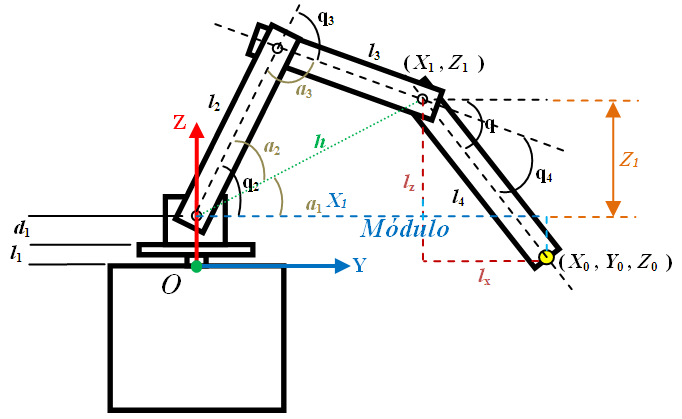
\includegraphics[scale=0.5]{EV/FIG.png}
 \end{center} \\
\section{Introducci�n}
\begin{flushleft}
�Qu� es y para que sirve? Como objetivo de esta actividad se espera conocer a profundidad de este tema en particular.\\ 

La convenci�n de Denavit Hartenberg o DH por sus siglas, es un procedimiento sistem�tico que sirve para describir la estructura cinem�tica de una cadena articulada constituida por articulaciones con un solo grado de libertad. \\

Para lograr comprender este procedimiento, se le sera explicado con un ejemplo gr�fico y anal�tico. 
\end{flushleft}\\

\section{Ejemplo Gr�fico}
Pondremos en contexto un brazo robotico con dos articulaciones solamente. \\

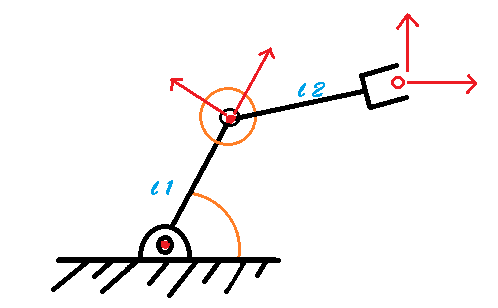
\includegraphics[scale=1]{EV/DH1.png} \\

Aunque lo parezca, la herramienta del robot (Pinza) no es una articulaci�n, es decir, en este caso no cuenta con grados de libertad.\\

Lo que se observa a simple vista es que se tienen dos articulaciones con sus respectivos grados de libertad. Por otro lado, vemos ya trazados ejes "X" y "Y" de ambas articulaciones.\\
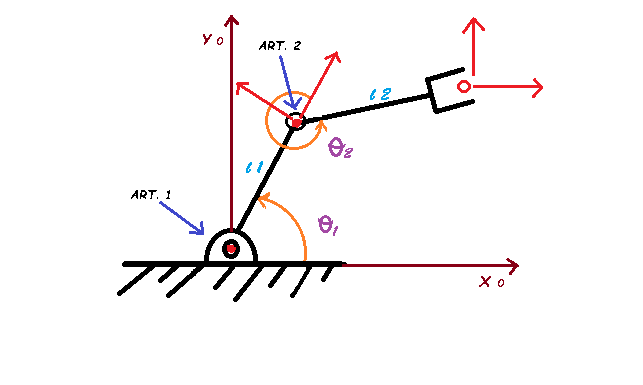
\includegraphics[scale=1]{EV/DH2.png} 

El numero de articulaciones ir�a en incremento a partir de uno dependiendo de cuantas sean, osea, a (n +1).\\

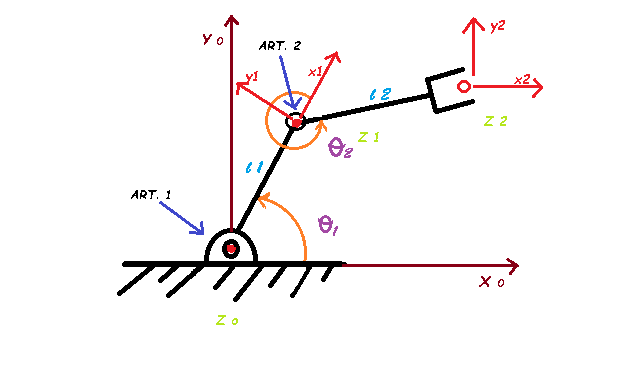
\includegraphics[scale=1]{EV/DH3.png} \\

ahora "z" ser� la posici�n en la que cada articulaci�n apunta, el cual vendr�a siendo b�sicamente la matriz de rotaci�n de cada articulaci�n con respecto a todas o independientemente si se trata de la primera.\\

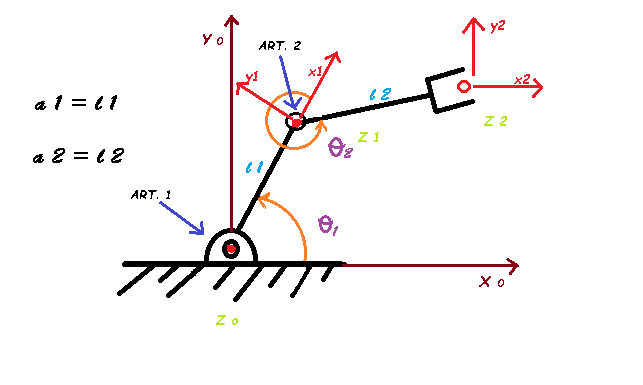
\includegraphics[scale=1]{EV/DH4.png} \\

Finalmente establezcamos algunas variables.

* C ser� Coseno\\
* S ser� Seno\\
* a ser� l, que a la vez es lo que mida.\\
* Teta, bueno,ser� el angulo de inclinaci�n, osea, una variable.\\ \\

Bien, tenemos dos articulaciones, la ultima depende de la anterior y as� sucesivamente y bueno, la tranformaci�n global de estas se dar�a de la siguiente manera... \\

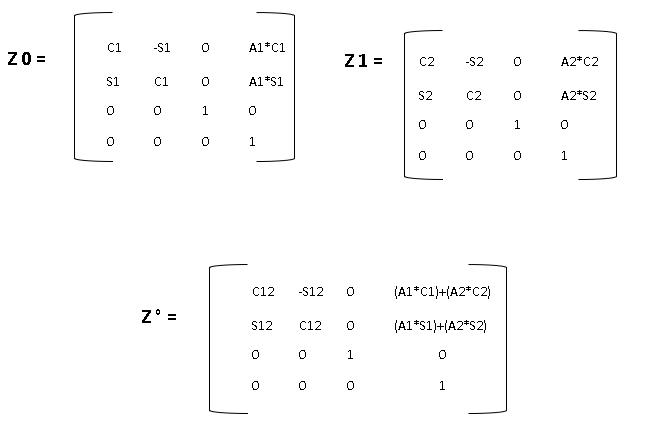
\includegraphics[scale=1]{EV/DH5.png} \\ 

"C12" se trata del ceno de teta uno mas teta dos, igualmente con el seno. \\

De esta manera se concluye el ejercicio. \\

\section{Conclusi�n}
Cuando vemos el proceso que se realizo con dos simples articulaciones, es f�cil darse cuenta de que al final, la posici�n rotacional final de cada articulaci�n depender�n de la anterior a ella, una tras otra, llegando al final del robot, empezando desde la base hasta la herramienta. 

\paragraph{\textbf{{\Large Referencias}}}

GIRALDO, Luis Felipe; DELGADO, Edilson; CASTELLANOS, Germ�n. Cinem�tica inversa de un brazo robot utilizando algoritmos gen�ticos. Revista Avances en Sistemas e Inform�tica, 2006, vol. 3, no 1, p. 29-34.

\end{document}